\documentclass[12pt,a4paper]{article}
\usepackage[utf8]{inputenc}
\usepackage[margin=1.5cm]{geometry}
\usepackage{amsmath}
\usepackage{mathtools}
\usepackage{amssymb}
\newcommand{\inter}{\begin{matrix}\prod\end{matrix}}

\begin{document}
\section*{Lezione 14}
\subsection*{INTERPOLAZIONE POLINOMIALE A TRATTI, CONVERGENZA E STABILITA', INTERPOLAZIONE SPLINE}
In questa lezione studieremo dei metodi di interpolazione che permettono di risolvere il problema della convergenza dell'interpolazione polinomiale, in particolare nel caso di un campionamento a passo costante (nodi equispaziati).\\ L'idea è, invece di prendere un unico polinomio interpolatore
con grado $\rightarrow\infty$, di costruire funzioni interpolanti polinomiali "\underline{a tratti}", ottenute "incollando" per continuità interpolatori di \underline{grado fissato} su una partizione dell'intervallo [a,b] in intervallini consecutivi.\\ Assumiamo che 
\begin{equation*}
    a=x_0<x_1<x_2<...<x_n=b
\end{equation*}
Il parametro che ci permette di infittire il campionamento sarà $h=max\Delta x_i$ dove $\Delta x_i= x_{i+1}-x_i$,\\$0\leq i\leq n-1$\\
Osserviamo che $h\rightarrow0\Rightarrow n\rightarrow\infty$ mentre il viceversa non vale in generale (è vero ad esempio però coi nodi equispaziati per cui $h=\frac{b-a}{n}$).\\ Infatti aumentando solamente il numero di nodi potremmo infittire in una parte dell'intervallo, senza aumentare l'informazione sulla funzione campionata nella parte restante
\begin{center}
    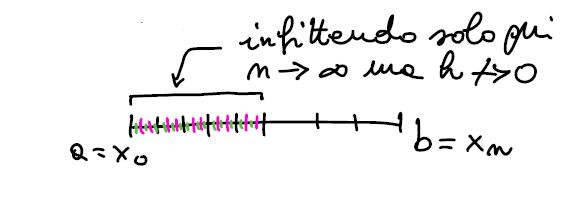
\includegraphics[scale=0.5]{calcolo.JPG}
\end{center}
\begin{minipage}{0.5\textwidth}
Per capire la tecnica iniziamo con un disegno dell'interpolazione
\begin{center}
    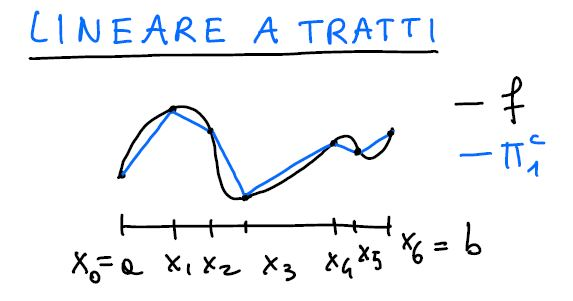
\includegraphics[scale=0.5]{calcolo2.JPG}
\end{center}
\end{minipage}
\begin{minipage}{0.5\textwidth}
$\ \ \ \ \ \ $ e qui sotto dell'interpolazione\\
\begin{center}
    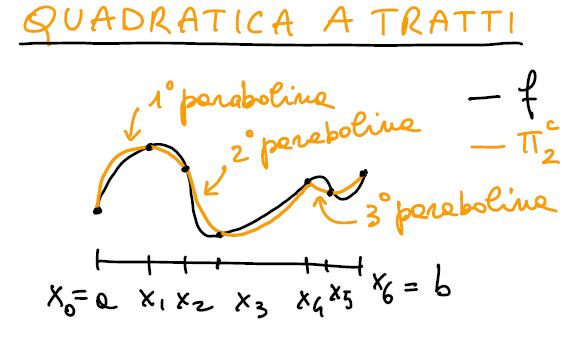
\includegraphics[scale=0.5]{calcolo3.JPG}
\end{center}
\end{minipage}\\
Nel primo caso l'interpolatore si ottiene tracciando i tratti di retta congiungenti i 2 punti del grafico corrispondenti a 2 nodi consecutivi. Nel secondo caso l'interpolatore si ottiene tracciando le "paraboline" corrispondenti a "pacchetti" di 3 nodi consecutivi (con un nodo di raccordo tra 2 pacchetti consecutivi) ovvero
\[\begin{split}
    x_0,x_1,x_2 & \rightarrow 1^\circ \text{ pacchetto}\\
    x_2,x_3,x_4 & \rightarrow 2^\circ \text{ pacchetto}\\
    x_4,x_5,x_6 & \rightarrow 3^\circ \text{ pacchetto}
\end{split}\]
Osserviamo subito che questo è possibile perché n=6 è pari.\\
In generale, per costruire una funzione interpolante di grado $s$ a tratti, abbiamo bisogno di pacchetti consecutivi di $s+1$ nodi distinti (che individuano un unico polinomio interpolatore "locale" di grado $s$), con un nodo di raccordo tra 2 pacchetti consecutivi.\\
Perché questo sia possibile bisogna che $n$ sia multiplo intero di $s$, cioè $n = k \cdot s$\\\\
\begin{minipage}{0.33\textwidth}
\begin{center}
    pacchetti\\
    $x_0, x_1, \dotso, x_s$\\
    $x_s, x_{s+1}, \dotso, x_{2s}$\\
    $x_{2s}, x_{2s+1}, \dotso, x_{3s}$\\
    $\dotso$\\
    $x_{(k+1) \cdot s}, \dotso, x_{ks}$
\end{center}
\end{minipage}
\begin{minipage}{0.33\textwidth}
\begin{center}
    tratti\\
    $[x_0, x_s]$\\
    $[x_s, x_{2s}]$\\
    $[x_{2s}, x_{3s}]$\\
    $\dotso$\\
    $[x_{(k-1) \cdot s}, x_{ks}]$
\end{center}
\end{minipage}
\begin{minipage}{0.33\textwidth}
\begin{center}
    interpolatori locali\\
    $\prod_{s,1}$\\
    $\prod_{s,2}$\\
    $\prod_{s,3}$\\
    $\dotso$\\
    $\prod_{s,k}$
\end{center}
\end{minipage}\\
La funzione interpolante, che chiameremo $\prod_s^c$ (interpolante "composta" di grado $s$ a tratti) \underline{non} è (in generale) un polinomio ed è ottenuta "incollando" per continuità nei nodi di raccordo i vari polinomi interpolatori locali di grado $s$, $\{ \prod_s, i\}$, $1 \leq i \leq k$.\\
Tale funzione polinomiale di grado $s$ a tratti è \underline{UNICA}, perché sono unici gli interpolatori locali $\prod_{s,i}$ e interpola perché $\forall x_j$ avremo che $x_j \in [x_{(i-1) \cdot s}, x_{is}]$ per un certo $i$ e quindi
\[
\forall j\, \inter_s^c (x_j) = \inter_{s,i} (x_j) = y_j = f(x_j)
\]
Osserviamo fra l'altro che per l'unicità se $f \in \mathbb{P}_m, \ m \leq s \ \Rightarrow \prod_s^c = f$ (cioè se $f$ è un polinomio di grado $\leq s$, allora l'interpolante a tratti di grado $s$ è quello stesso polinomio).\\
Rispetto all'interpolazione con un unico polinomio $\prod_n$ il cui grado $n$ viene mandato ad $\infty$, l'aspetto chiave nella costruzione di $\prod_s^c$ è che $s$ è \underline{fissato} (e per infittire il campionamento si prende\\
$h=max \ \Delta x_i \to 0$, in modo da infittire in tutto l'intervallo $[a,b]$).\\
Il caso dei nodi equispaziati rientra nella costruzione con
\[
x_i = a+ih, \ 0 \leq i \leq n, \ h = \frac{b-a}{n}
\]
e corrisponde ad infittire a passo costante il campionamento (ma la costruzione è possibile per qualsiasi distribuzione di $n+1$ nodi purché $n$ sia multiplo di $s$).\\
Il vantaggio dell'interpolazione polinomiale a tratti è che garantisce la \underline{convergenza uniforme}, cioè 
\[
dist(f, \inter_{s}^{c}) \to 0, \ h \to 0
\]
Enunciamo ora, e dimostriamo per $s=1$, un risultato generale sulla convergenza (e sull'ordine
di infinitesimo dell'errore in $h$)\\\\
\textbf{TEOREMA (convergenza uniforme dell'interpolazione polinomiale a tratti)}\\
\begin{center}
    \fbox{\begin{minipage}[t]{15cm}%
        Siano $f \in C^{s+1}[a,b], \ s \geq 0$ e $\{x_i \} \subset [a,b] \ n+1$ nodi distinti, con $n$ multiplo di $s$
        \begin{center}
            allora
        \end{center}
        \begin{center}
            $\exists k_s > 0: \ dist(f, \prod_s^c) \leq k_s \cdot h^{s+1}, \ h = max \ \Delta x_i$
        \end{center}
    \end{minipage}}
\end{center}

\textbf{Dimostrazione}\\
Dimostriamo il teorema per $s=1$ (interpolazione lineare a tratti)\\
Osserviamo che
\[ \begin{split}
    dist(f, \inter_{1}^{c}) & = \max_{x \in [a,b]} |f(x) - \inter_{1}^{c} (x) | \\
    & = \max_{0 \le i \le n-1}\, \max_{x \in [x_i, x_{i+1}]} |f(x) - \inter_{1}^{c} (x) |
\end{split} \]
(perché il max su tutto [a,b] è il massimo dei max sui singoli intervallini)
\[= \max_{1 \le i \le n}\, \max_{x \in [x_{i-1},x_i]} |f(x) - \inter_{1,i}^{}(x)|\]
(perché in $[x_{i-1, x_i}] \,\prod_1^c$ è il polinomio interpolatore locale di grado 1 $\prod_{1,i}$ su $(x_{i-1}, y_{i-1})$ e $(x_i, y_i)$).\\
Ora ricordando la stima dell'errore di interpolazione polinomiale a grado $s$ ricavata dalla scorsa lezione
\[\max_{x\in [\alpha , \beta]}|f(x) - \inter_{s}^{}(x)| \le \max_{x\in [\alpha , \beta]}|f^{(s+1)}(x)|\cdot\frac{h^{s+1}}{4(s+1)} \]
valida per $f \in C^{s+1}[\alpha, \beta]$ e $h = \frac{b-a}{s}$, e applicandola per $s=1$ e $[\alpha,\beta] = [x_{i-1},x_i]$, otteniamo
\[\max_{x\in [x_{i-1},x_i]}|f(x) - \inter_{1,i}^{}(x)| \le \max_{x\in [x_{i-1},x_i]}|f''(x)|\cdot\frac{h^2}{8} = M_{2,i} \frac{h^2}{8} \]
da cui
\[ \begin{split}
    dist(f, \inter_{1}^{c}) & = \max_{1 \le i \le n}\, \max_{x \in [x_{i-1},x_i]} |f(x) - \inter_{1,i}^{}(x)| \\
    & \le \frac{h^2}{8} \max_{1 \le i \le n} M_{2,i} \\
    & = \frac{M_2}{8}h^2
\end{split} \]
con $M_2 = \max_{x\in[a,b]} |f''(x)|$ (di nuovo perchè il $\max$ di $|f''(x)| \; m[a,b]$ è il massimo dei $\max$ di $|f''(x)|$ sui singoli intervallini).\\
\textbf{...fine dimostrazione}\\\\
Vale la pena di notare che l'interpolazione lineare a tratti converge anche se $f \in C^1[a,b]$ con $dist(f,\inter_1^c)\leq ch, \; c>0$, e perfino per $f$ solo continua in $[a,b]$, anche se in questo caso si sa solo che $dist(f,\inter_1^c) \rightarrow 0$, $h \rightarrow 0$ (non facciamo le dimostrazioni).\\
La dimostrazione fatta per $s=1$ si può adattare facilmente: $s>1$ nel caso di modi equispaziati, ottenendo $K_s=\dfrac{M_{s+1}}{4(s+1)}$ (dimostrazione facoltativa).\\
Possiamo dire qualcosa anche sulla stabilità dell'interpolazione polinomiale a tratti, sempre nel caso di nodi equispaziati che sappiamo essere fortemente instabile per l'intepolazione polinomiale standard.\\
Infatti, detta $\widetilde{\inter_1^c}$ l'interpolante a tratti costruita sui valori approssimati $\{\tilde{y_i}\}$, con $\max|y_i-\tilde{y_i}|\leq \varepsilon$:
\[
dist(\inter_s^c,\widetilde{\inter_s^c})=\max_{1 \le i \le n}\, \max_{x \in [x_{i-1},x_i]} | \inter_s^c(x)-\widetilde{\inter_s^c}(x)| \]
\[= \max_{1 \le i \le n}\, \max_{x \in [x_{i-1},x_i]} | \inter_{s,i}^{}(x)-\widetilde{\inter_{s,i}^{}}(x)|\leq \Lambda_s^{eq}\cdot \varepsilon\]
perchè $\max | \inter_{s,i}(x)-\widetilde{\inter}_{s,i}(x)|\leq \Lambda_s^{} \cdot \varepsilon$, con $x \in [x_{i-1},x_i]$ dove $\Lambda_s^{eq}$ è la costante di Lebesgue per grado $s$, cioè:
\[
	\Lambda_s^{eq} \approx \dfrac{2}{e} \cdot \dfrac{2^s}{s \log(s)} \text{, con } s>1 \text{ fissato}
\]
Ora, se $s$ non è grande (le interpolazioni a tratti più usate sono la lineare, quadratica e cubica, cioè con $s=1,2,3$) la costante di Lebesgue è relativamente piccola e quindi l'interpolazione \underline{a tratti} su nodi \underline{equispaziati} è sostanzialmente \underline{STABILE}, perchè il coefficiente di amplificazione dell'errore sui dati dipende da $s$ ma \underline{non} da $n$ (mentre nell'interpolazione polinomiale standard $\Lambda_n \sim \dfrac{2}{e} \cdot \dfrac{2^n}{n \log(n)}$, con $n \to \infty$).\\
Come abbiamo visto, l'interpolazione polinomiale a tratti è una tecnica efficace per la ricostruzione di funzioni da dati discreti (vedremo che la garanzia di convergenza sarà importante, ad esempio, per ricavare formule di approssimazione di integrali definiti, a partire da un campionamento della funzione integranda).\\
C'è però un problema di fondo che la rende poco adatta ad esempio ad applicazioni nella grafica al computer (a meno che $h$ non sia molto piccolo), ed è il fatto che in generale $\inter_s^c$ è solo continua (i nodi di raccordo tra pacchetti sono punti angolosi). Basta infatti pensare a come sono fatte le interpolanti lineare e quadratica a tratti:
\begin{center}
    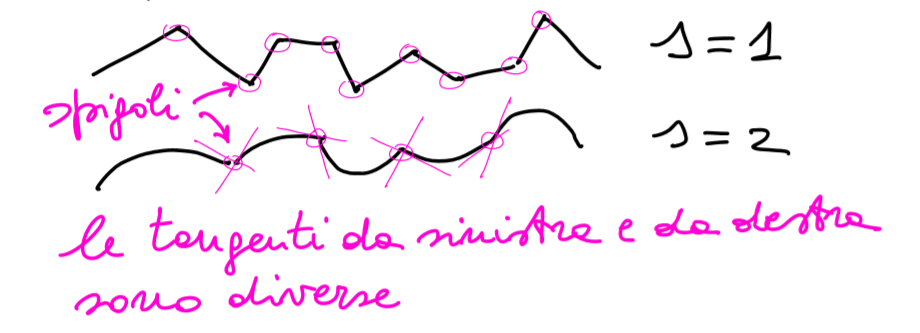
\includegraphics[scale=0.4]{img_pag18.png}
\end{center}
Nelle applicazioni grafiche servono invece spesso interpolanti ``lisce", che permettono di disegnare curve senza spigoli ``artificiali".\\
Questo non è ottenibile con la tecnica fin'ora descritta, ma fino agli anni '50 sono state sviluppate tecniche alternative che potessero garantire nello stesso tempo convergenza e assenza di spigoli (o regolarità di ordine anche superiore).\\
Una di queste tecniche, nata all'inizio per la progettazione nel campo dell'industria automobilistica, navale e aereonautica, si chiama interpolazione polinomiale a tratti di tipo \underline{SPLINE}.\\
Ne faremo di seguito alcuni cenni, senza dimostrazioni, per capire l'idea del metodo. \\
Data $f \in C[a,b]$ e $n+1$ punti $\left\{ (x_i,y_i) \right\}_{0 \leq i \leq n}$, $y_i=f(x_i)$, con $a=x_0 < x_1 < x_2 <\dots<x_n=b$, una funzione polinomiale a tratti interpolante si chiama interpolante \underline{spline} di grado $k$, indicata con $S_k(x)$, se valgono le seguenti condizioni:
\begin{enumerate}
    \item $S_k(x_i)=y_i$, $0 \leq i \leq n$ (vincoli di interpolazione)
    \item $S_k \vert_{I_i} \in \mathbb{P}_k$, $I_i=[x_i,x_{i+1}]$ e $0 \leq i \leq n-1$ ($S_k$ ristretta all'$i$-esimo intervallino tra i nodi consecutivi è un polinomio di grado $\leq  k$)
    \item $S_k \in C^{k-1}[a,b]$ (vincolo di regolarità)
\end{enumerate}
Osserviamo subito che $S_1=\inter_1^c$, cioè una spline lineare è in realtà l'interpolazione lineare a tratti che già conosciamo, ed è quindi completamente determinata dai vincoli (ma è solo continua). Le spline "lisce", cioè con alcune derivate continue, partono da $k=2$: spline quadratiche, spline cubiche, \dots \\
E' importante ribadire che le spline \underline{non} sono in generale polinomi, ma sono funzioni polinomiali a tratti, con la differenza sostanziale rispetto all'interpolazione a tratti standard che i nodi non sono raggruppati a "pacchetti", perché la spline è localmente un polinomio tra due nodi consecutivi (non c'è quindi la restrizione che $n$ sia multiplo di $k$) e che viene ottenuta "incollando" tra di loro i vari polinomi locali imponendo che i raccordi siano "lisci" (le derivate nei punti di raccordo, che sono tutti i nodi interni, sono vincolate ad essere continue fino ad un certo ordine) \\ Per capire come funziona in pratica la costruzione di una interpolante spline, trattiamo il caso $k=3$ (SPLINE CUBICHE), che sono le spline più usate nelle applicazioni, cominciando con un disegno esplicativo
\begin{center}
    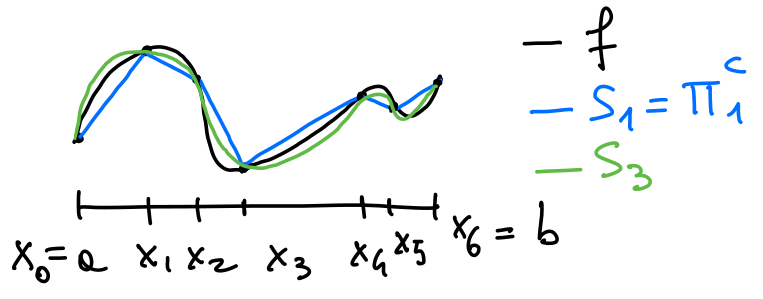
\includegraphics[scale=0.4]{img_pag23.png}
\end{center}
Quali sono i vincoli per $S_3$ e quali i parametri da determinare?\\
Innanzitutto osserviamo che in $1_i=[x_i,x_{i+1}]$ $S_3(x)$ è un polinomio cubico, cioè ha la forma 
\begin{equation*}
    S_3 \vert _{I_i} = p_{3,i} = a_{0,i} + a_{1,i}x + a_{2,i}x^2 + a_{3,i}x^3
\end{equation*}
Ci sono quindi 4 coefficienti incogniti per ciascuno degli $n$ intervallini, quindi le \underline{incognite} sono in tutto 4 $n$. \\
E i vincoli?
\begin{align*}
 & S_3(x_0)=p_{3,1}(x_0)=y_0 \\ 
 & S_3(x_n)=p_{3,n}(x_n)=y_n\\ 
 & p_{3,i}(x_i)=y_i=p_{3,i+1}(x_i), \ 1 \leq i \leq n-1 
\end{align*}
questi vincoli assicurano interpolazione e continuità, restano i vincoli di regolarità\\
\begin{center}
$\begin{matrix}
p_{3,i}'(x_i) = p_{3,i+1}'(x_i)\\
p_{3,i}''(x_i) = p_{3,i+1}''(x_i)
\end{matrix}$
$\biggl\}1 \leq i \leq n-1 \ \longleftarrow \ $ $2(n-1)$ vincoli 
\end{center}
generati dalla richiesta che $S_3$ sia globalmente $C^2$\\ 
Quindi in tutto ci sono 
\begin{equation*}
    2 + 2(n-1) + 2(n-1) = 4n-2
\end{equation*}
vincoli, che diventano altrettante equazioni.\\
Di che tipo di equazioni si tratta ? Siccome le incognite sono i coeff. degli $n$ polinomi cubici $\{P_{3,i}\}$, che entrano \underline{linearmente} nelle corrispondendi equazioni (perchè i polinomi e le loro derivate sono combinazioni lineari dei monomi $x^j$ e delle loro derivate, le derivate sono infatti negli spazi di funzioni derivabili, $\frac{d^m}{dx^m}(\alpha f(x) + \beta g(x)) = \alpha \frac{d^m}{dx^m} f(x) + \beta \frac{d^m}{dx^m} g(x) $, alla fine i vincoli diventano un SISTEMA LINEARE di 4 $n-2$ equazioni in 4 $n$ incognite. \\
Tale sistema non è determinato (è sottodeterminato, ci sono meno equazioni che incognite, quindi può avere $\infty$ soluzioni).\\
Per determinare la soluzione (cioè i coefficienti locali della $S_3$) bisogna imporre 2 vincoli aggiuntivi in modo che il sistema diventi quadrato ($4n \times 4n$) e non singolare (per avere $\exists!$).\\
Ci sono vari set di coppie di condizioni  aggiuntive che si può dimostrare che garantiscono una matrice $4n \times 4n$ non singolare (cioè invertibile; non faremo queste dimostrazioni).\\
Ad esempio le condizioni 
\begin{equation*}
    S_3''(x_0)=p_{3,1}''(x_0)=0=p_{3,n}''(x_n)=S_3''(x_n)
\end{equation*}
(derivate seconde nulle agli estremi) oppure le condizioni
\[
p'''_{3,1}(x_1) = p'''_{3,2}(x_1), \ p'''_{3,n-1}(x_{n-1}) = p'''_{3,n} (x_{n-1})
\]
($S'''_3$ continua nel secondo e nel penultimo nodo).\\
Quest'ultima coppia di vincoli permette di costruire le cosiddette "spline naturali" che sono quelle implementate ad esempio automaticamente in Matlab quando si usa il comando SPLINE passando in input i vettori $\{x_i \}$ e $\{ y_i \}$.\\
Di nuovo, come per l'interpolazione a tratti standard, vale la pena di ribadire che per l'unicità dell'interpolante spline cubica,
\[
f \in \mathbb{P}_m, \ m \leq 3 \Rightarrow S_3 = f
\]
Non ci occuperemo dell'effettiva implementazione dell'interpolazione spline (ci sono tecniche alternative alla costruzione e soluzione del sistema lineare), discutiamo invece l'aspetto chiave dopo aver fatto vedere che la costruzione algebrica si può fare in modo univoco, che è il problema della \underline{convergenza}.\\\\
Daremo ora (senza dimostrarlo, la dimostrazione è complicata) un risultato di convergenza per le $S_3$, con gli ordini dell'errore in $h$, dove $h = max \ \Delta x_i$.\\
\textbf{TEOREMA (convergenza uniforme dell'interpolazione spline cubica)}\\
\begin{center}
    \fbox{\begin{minipage}[t]{15cm}%
        Siano $f \in C^4 [a,b]$ e $\{ x_i \} \subset [a,b] \ n+1$ nodi equispaziati $(h = \frac{b-a}{n})$
        \begin{center}
            allora
        \end{center}
        \begin{center}
            $\exists k_{3,j} > 0: \ dist_{0 \leq j \leq 3}(f^{(j)}, S_3^{(j)}) \leq k_{3,j} \cdot h^{4-j}$
        \end{center}
    \end{minipage}}
\end{center}
Osserviamo innanzitutto che l'ordine di infinitesimo di $dist(f, S_3)$ è $h^4$, che è lo stesso che si otterrebbe con $\inter_3^c$ (che è costruibile però solo se $n$ è multiplo di 3, mentre con $S_3$ non ci sono vincoli su $n$).\\
Ma c'è di più: $S_3 \in C^2 [a,b]$ per costruzione, e risulta che
\[
\begin{split}
    dist(f', S'_3) \leq k_{3,1} \cdot h^3 \\
    dist(f'', S''_3) \leq k_{3,2} \cdot h^2
\end{split}
\]
e addirittura
\[
dist(f''', S'''_3) \leq k_{3,3} \cdot h
\]
cioè non solo $S_3$ converge uniformemente ad $f$, ma anche le sue derivate fino alla terza convergono alla corrispondente derivata di $f$ (si noti che $S_3$ è cubica a tratti, $S'_3$ è quadratica a tratti, $S''_3$ è lineare a tratti e $S'''_3$ è costante a tratti).\\
Per capirlo basta pensare che localmente si tratta di derivare un polinomio di grado 3, $p_{3,i} (x) \ 1 \leq i \leq n$.\\
È importante però dire che mentre $S_3$ appossima $f$ interpolandola $(S_3 (x_i) = y_i \forall i)$ le sue derivate $S_3^{(j)}$ approssimano le $f^{(j)}, \ 1 \leq j \leq 3$, ma non le interpolano ($S_3$ non è costruita per interpolare le derivate di $f$ ma per essere "liscia", nella fattispecie di regolarità di $C^2$; ciononostante, il vincolo di regolarità porta a poter approssimare anche le derivate di $f$).\\
Infine cosa si può dire della stabilità? Si può dimostrare che come nel caso di $\prod_3^c$ le $S_3$ sono stabili, cioè detta $\Tilde{S}_3$ la spline cubica costruita su valori affetti da errore $\Tilde{y}_i$ con 
\[\max |y_i - \Tilde{y}_i| \le \varepsilon\]
si ha \[dist(\Tilde{S}_3, S_3) \le c \cdot \varepsilon\]
per una opportuna costante $c>0$.\\
Invece le derivate di $S_3$ non sono stabili per $\varepsilon$ fissato e $h \to 0$, perchè viene ereditata la sostanziale instabilità delle operazioni funzionali di derivazione (come vedremo della lezione 17 sulla "derivazione numerica").\\
Per concludere possiamo ribadire che l'interpolazione a tratti (standard o spline) risolve il problema della convergenza su distribuzioni arbitrarie di nodi ( purché $h=max\Delta x_i \rightarrow 0$ e per nodi non equispaziati con la condizione tecnica aggiuntiva che il rapporto $\frac{max\Delta x_i}{min\Delta x_i}$ resti limitato);\\
ad esempio c'è convergenza per la funzione dell'esempio di Runge con nodi equispaziati su $[a,b]=[-5,5]$:\\
\begin{center}
    $dist(\frac{1}{1+x^2}, \underset{\underset{\inter^1_c}{\shortparallel}}{S_1}) \leq M_2 \frac{h^2}{8}$
\end{center}
e nel caso cubico: 
\begin{center}
$dist(\frac{1}{1+x^2},S_3)\leq k_{3,0} h^4$\\
\end{center}
Queste stime fatte per $f \in C^\infty$ ci permettono fra l'altro di capire che una volta scelto il grado $k$ dell'interpolazione a tratti, l'errore resta in generale di ordine $k+1$ in $h$ anche se $f \in C^m [a,b]$ con $m > k+1$ (ad esempio, l'errore dell'interpolazione lineare a tratti resta di ordine $h^2$ anche se $f \in C^\infty$)

\end{document}
